\begin{figure}
    \centering\footnotesize
    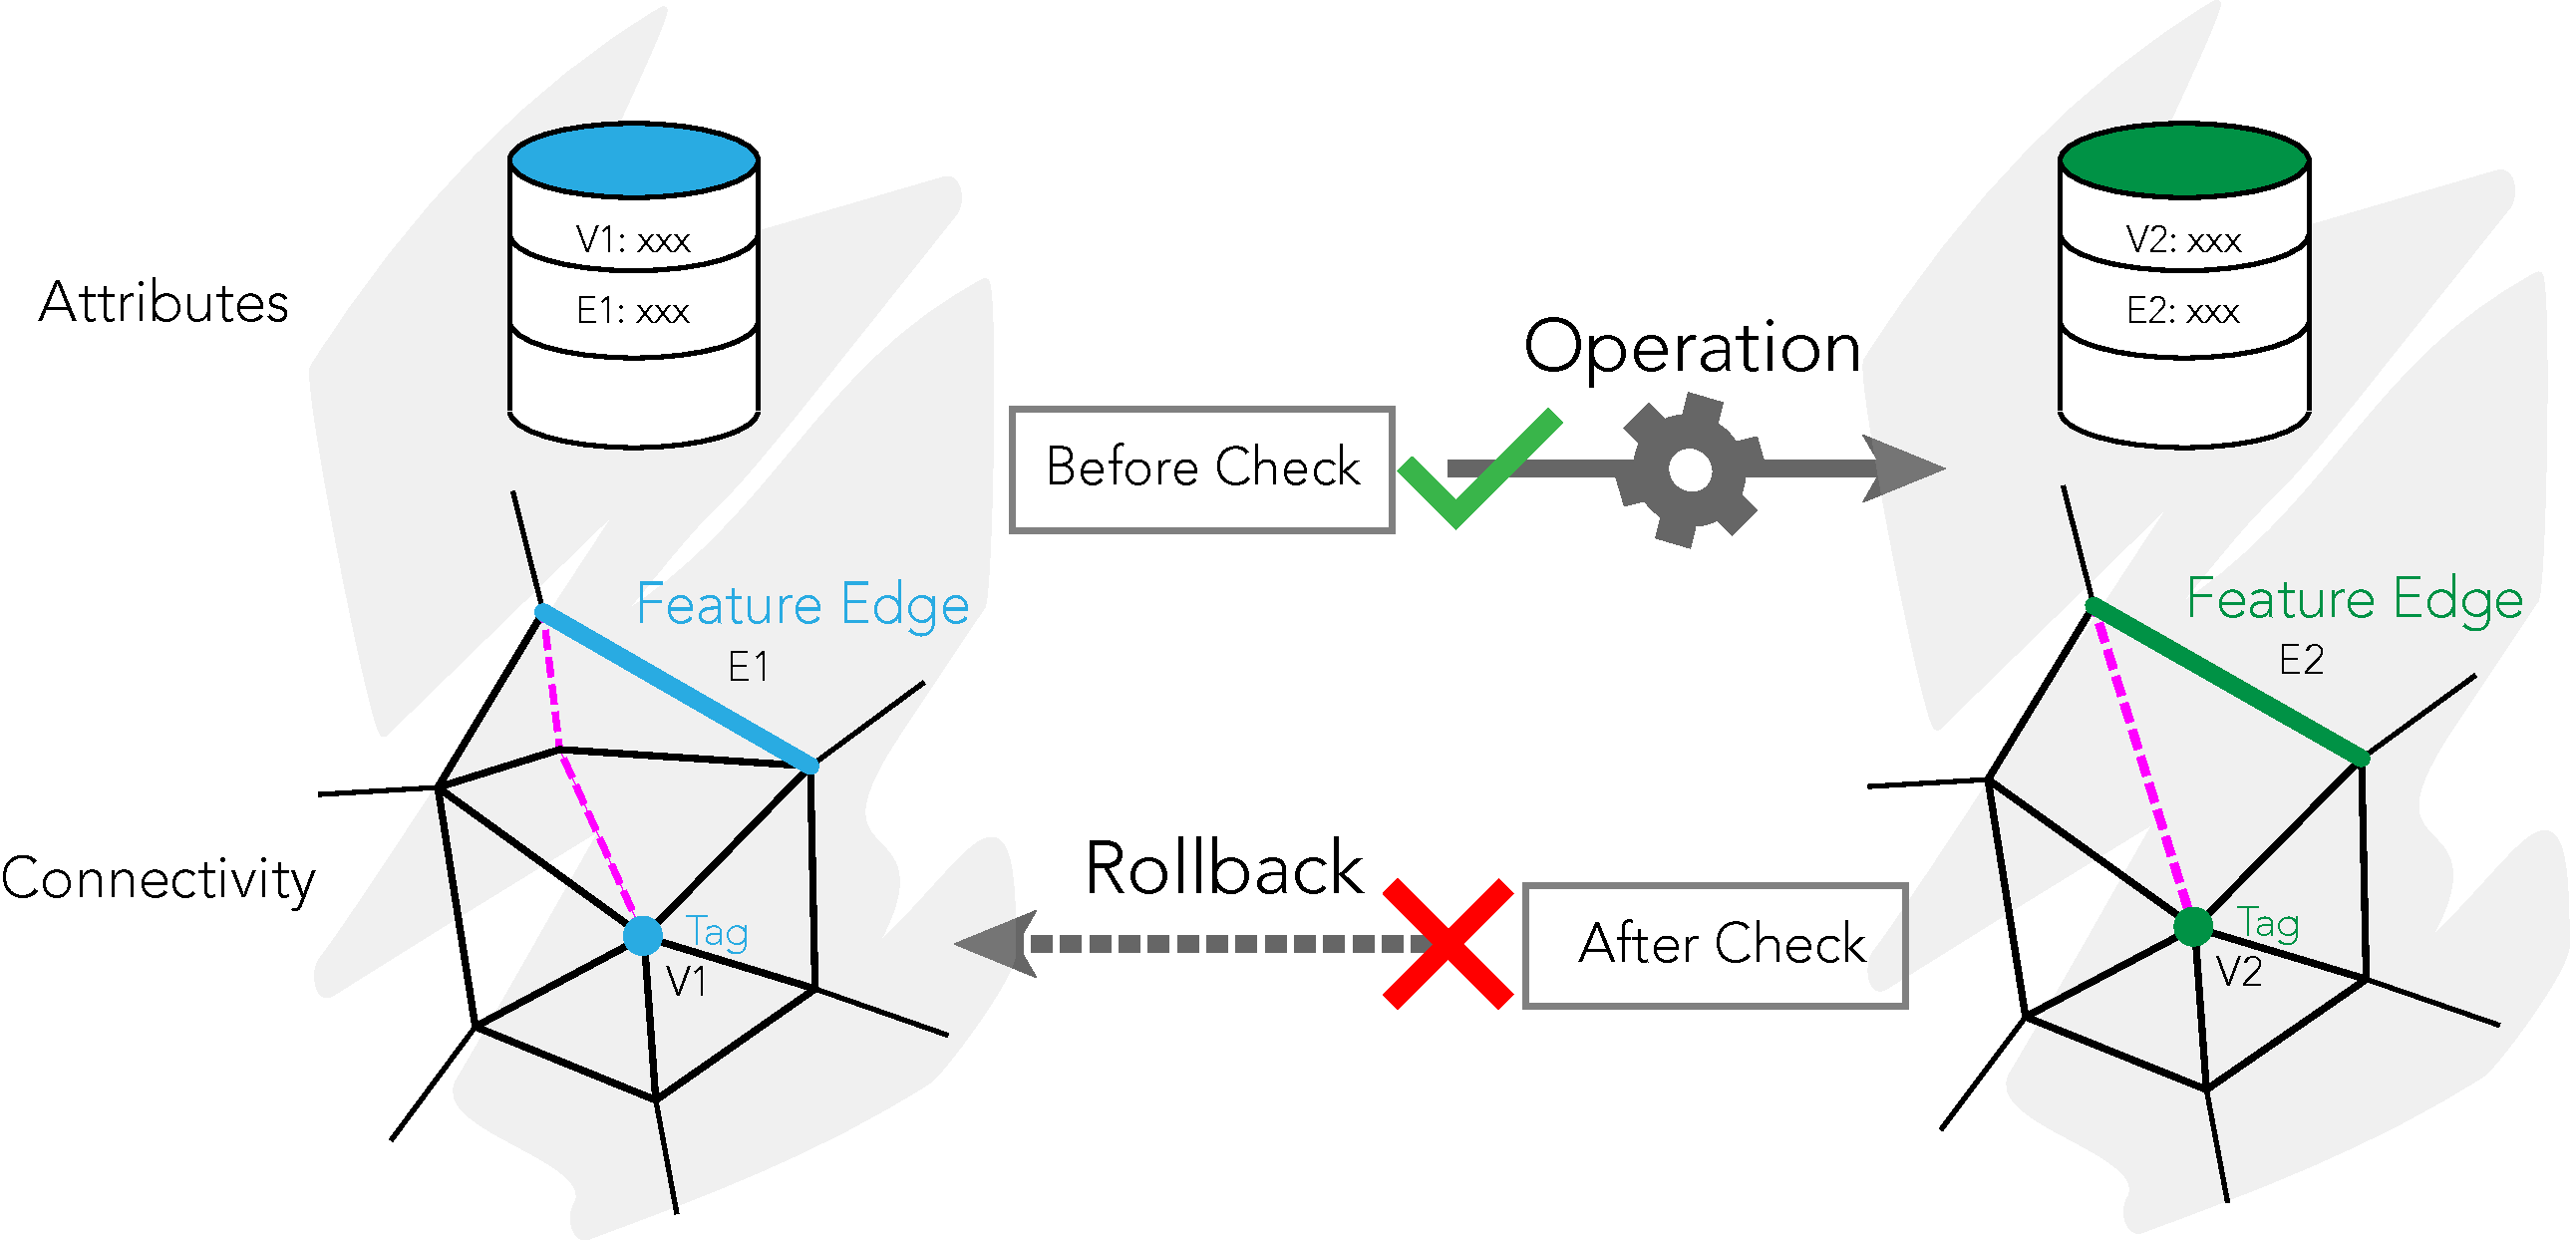
\includegraphics[width=\linewidth]{wmtk-tex/figs/pipeline_illustration.pdf}
    \caption{{Overview of the components behind our specification. A mesh is represented trough its topology, implemented by our library, and a list of user provided attributes. Before an operation is attempted, we explicitly perform a pre-check, and, if successful, we generate a mesh (attributes and topology). At this point, we trigger the after check to validate the operation (e.g., check if the newly generate mesh has positive volume). In case the after check fails, we \emph{automatically} rollback the operation and restore the mesh to its previous \emph{valid} state.}}
    \label{fig:pipeline}
\end{figure}

\section{Method}

Our declarative specification is designed to remove the burden of low-level management of the mesh connectivity {and attributes}, allowing an algorithm designer to focus only on high-level requirements. The design consists of five components. 

\subsection{{Mesh editing components}}

\paragraph{Operation Rollback.}
It is common to perform mesh editing to improve a given energy functional, such as mesh quality or element size. However, due to the discrete nature of the operations, it is not possible to use standard smooth optimization techniques, and instead the effect of the energy is evaluated before and after every operation to measure its effect on the energy. This is commonly implemented using an ad-hoc energy evaluation that ``simulates'' the operation only for the purpose of measuring the energy change. This simulation is complex (especially in 3D), and error-prone, as not only the connectivity changes, but the energy likely depends on properties attached to mesh elements, which needs to be updated accordingly.

We propose instead to make this process {opaque} to the user, providing to the user-code an explicit copy of the  mesh (and up to date attributes) \emph{before and after} the operation is performed to allow an easy and reliable energy evaluation. The correctness and efficiency of this process is handled by the runtime. This reduces the complexity of mesh editing considerably in our experience, as it makes them more similar to traditional finite difference approaches where the energy is evaluated on different points on the domain to approximate its derivative.

\paragraph{Explicit Invariants.}
It is common to have a set of desiderata on the mesh that needs to be satisfied, such as avoiding triangle insertions or self-intersections. Given the complexity of a mesh editing algorithm it is difficult to ensure that they are satisfied, as these conditions needs to be checked after every operation is applied (and they often depend on attributes too, such as vertex positions).

We propose to make these invariants explicit, and delegate to the library the task of ensuring that they are checked after every mesh modifications, and after the input is loaded. In this way, not only the code is simpler, but it is much easier to ensure correctness, as the checks are handled transparently by the library.

\paragraph{Explicit Attribute Update.}
Mesh attributes are usually handled by low-level meshing libraries, allowing to attach them to the desired mesh element (vertex, edge, face, triangle, or tetrahedra). However, the handling of attributes after a local operation is performed is usually a responsibility of the user code, as it is dependent on the application. 

We propose to make this process more explicit, requiring the user to provide the rules on how to update attributes after operation in a high-level specifications, and delegating the actual update to the library. This makes the specification more direct and less error-prone, and allows users to write algorithms without having to know the low-level details on how the local mesh operations work.

\paragraph{Parallel Scheduling.}
The type and scheduling of local operations is crucial in mesh editing algorithms. It usually involves maintaining a priority queue of operations, which is updated after every local operation.

We provide a direct way of controlling the operations performed and how the queue is updated. In the library, we can then distribute the work automatically on multiple threads, hiding from the user code the complexity of performing mesh editing operations in parallel and ensuring that race conditions are avoided. 

\paragraph{Abstract Mesh Navigation.}
Both invariant and attribute updates require navigating a mesh. Instead of relying on data-structure specific navigation, we favor the use of the cell tuple abstraction \cite{Brisson1989}. This allows the specification to be independent of the mesh data structure used in the library. The \texttt{Tuple} stores four indices  (three for surface meshes), vertex, edge, face, and tetrahedron and provides a single function per index, called \texttt{switch}, to change one index while keeping the other indices fixed. For instance \texttt{switch\_vertex} changes the vertex index while keeping edge, face, and tetrahedron fixed which has the effect of selecting the opposite vertex on an edge.

%%%%%%%%%%%%%%%%%%%%%%%%%%%%%%%%%%%%%%%%%%%%%%%%%%%%%%%%%
\subsection{Declarative Specification}

%As aforementioned explained, the key idea of our declarative specification is to decouple the low-level implementation details from the logic of the actual algorithm. 
%The key idea is to provide an high-level API hiding the complexity for topology changes, and delegate to the application code the update of vertex, edge, face, and tetrahedron attributes. For instance, our meshes do not store any geometric information such as vertex positions. 

Our API provides two abstractions: a \texttt{TetMesh} (and \texttt{TriMesh} class for 2D) (Algorithm \ref{algo:tetmesh}), and a \texttt{Scheduler} (Algorithm~\ref{algo:scheduler}).

\begin{algorithm}
\inputminted{cpp}{wmtk-tex/code/tetmesh.cpp}
\caption{API of our \texttt{TetMesh} class.}
\label{algo:tetmesh}
\end{algorithm}

% \begin{algorithm}
% \inputminted{cpp}{wmtk-tex/code/trimesh.cpp}
% \caption{API of our \texttt{TriMesh} class.}
% \label{algo:trimesh}
% \end{algorithm}


\begin{algorithm}
\inputminted{cpp}{wmtk-tex/code/scheduler.cpp}
\caption{API of our \texttt{Scheduler}.}
\label{algo:scheduler}
\end{algorithm}

\paragraph{Mesh Classes}
Both the \texttt{TetMesh} and \texttt{TriMesh} classes provide the basic local operations (e.g., edge split or collapse) and, for each operation, their corresponding \emph{before} and \emph{after} methods. The mesh class is responsible of implementing the operations changing the topology, and the application code must \emph{only} override the before and after methods to update attributes. The before method has a view of the mesh before the operation, and can thus navigate it to cache local attributes, while the after method has a view after the operation is performed, and it is responsible for updating attributes. In the simple case of regular subdivision of a triangle mesh, the \texttt{split\_before} caches the coordinates of the two edge endpoints, and the \texttt{split\_after} computes the position of the newly inserted vertex by averaging them. 

In addition, the mesh class provides a method, which can be overridden by the user code, that \emph{automatically} verifies user-provided invariants (e.g., maintain positive elements' volume). All user-provided methods return a Boolean status to notify the mesh classes if the operation fails; in case it does, our API rolls back the operation and restores the topology to the previous valid state. As the connectivity and attributes management is handled by the class, this ensures that, in case of failure of the operation, the mesh will go back to a valid state.

Our API provides the standard local operations: edge collapsing. edge/face swapping, edge splitting, and smoothing. We also provide an additional, non standard, operation: triangle insertion. This operation is an enhanced version of splitting where multiple edges, faces, and tetrahedra are subdivided to represent an input  triangle provided as input. This operation is useful to compute mesh arrangements, and it is also used in meshing algorithms \cite{Hu:2019:fTetWild}.

Since the \texttt{TetMesh} class only handles topology, the operation requires the list of edges and tetrahedron the input triangle intersects. Internally it subdivides all of them, and generates a valid tetrahedral mesh using the connectivity table in~\cite{Hu:2019:fTetWild}. The before operation provides the user the list of  faces that will be changed by the operation, allowing the user code to explore the mesh and cache attributes,  while the after provides a mapping between the old faces and any newly inserted face in the mesh.


\paragraph{Scheduler}
The second part of our API is the \texttt{Scheduler} that is responsible to control the order of the individual operations and then execute a list of operations. The main purpose of the scheduler is to abstract the operation order and hide parallelization details from the user. Our scheduler provides customizable callbacks, including,
\begin{itemize}
    \item \emph{Priority} to order the local mesh edit operations.
    \item \emph{Renew neighbor tuples} that is invoked after a successful operation, to add newly created tuples and operations into the queue.
    \item \emph{Lock vertices} that provides information on the affected region for the operation, and avoiding conflicts.
    \item \emph{Stopping criterion} that is checked periodically to terminate the program if certain criterion is met. For example, number of vertices, or quality criterion.
\end{itemize}




% \paragraph{Harmonic Tetrahedralization}
% \TODO{write me}


\subsection{Implementation.}

We implement a runtime for our specification in C++, using Intel oneTBB for parallelization.

\paragraph{Data Structure.} We opt for an indexed data structure, where we explicitly represent the vertices and the simplex of higher dimension (triangle for 2D, tetrahedra for 3D). Each vertex explicitly stores a list of incident simplices, and each simplex stores a sorted list of its vertices. While not the most efficient option for navigation, this data structure makes the implementation of local operation much simpler. 

\paragraph{Parallelization.} To avoid conflicts between local operations working on the same part of the mesh, we introduce a synchronization mechanism using locks. 

\begin{figure}\centering\footnotesize
    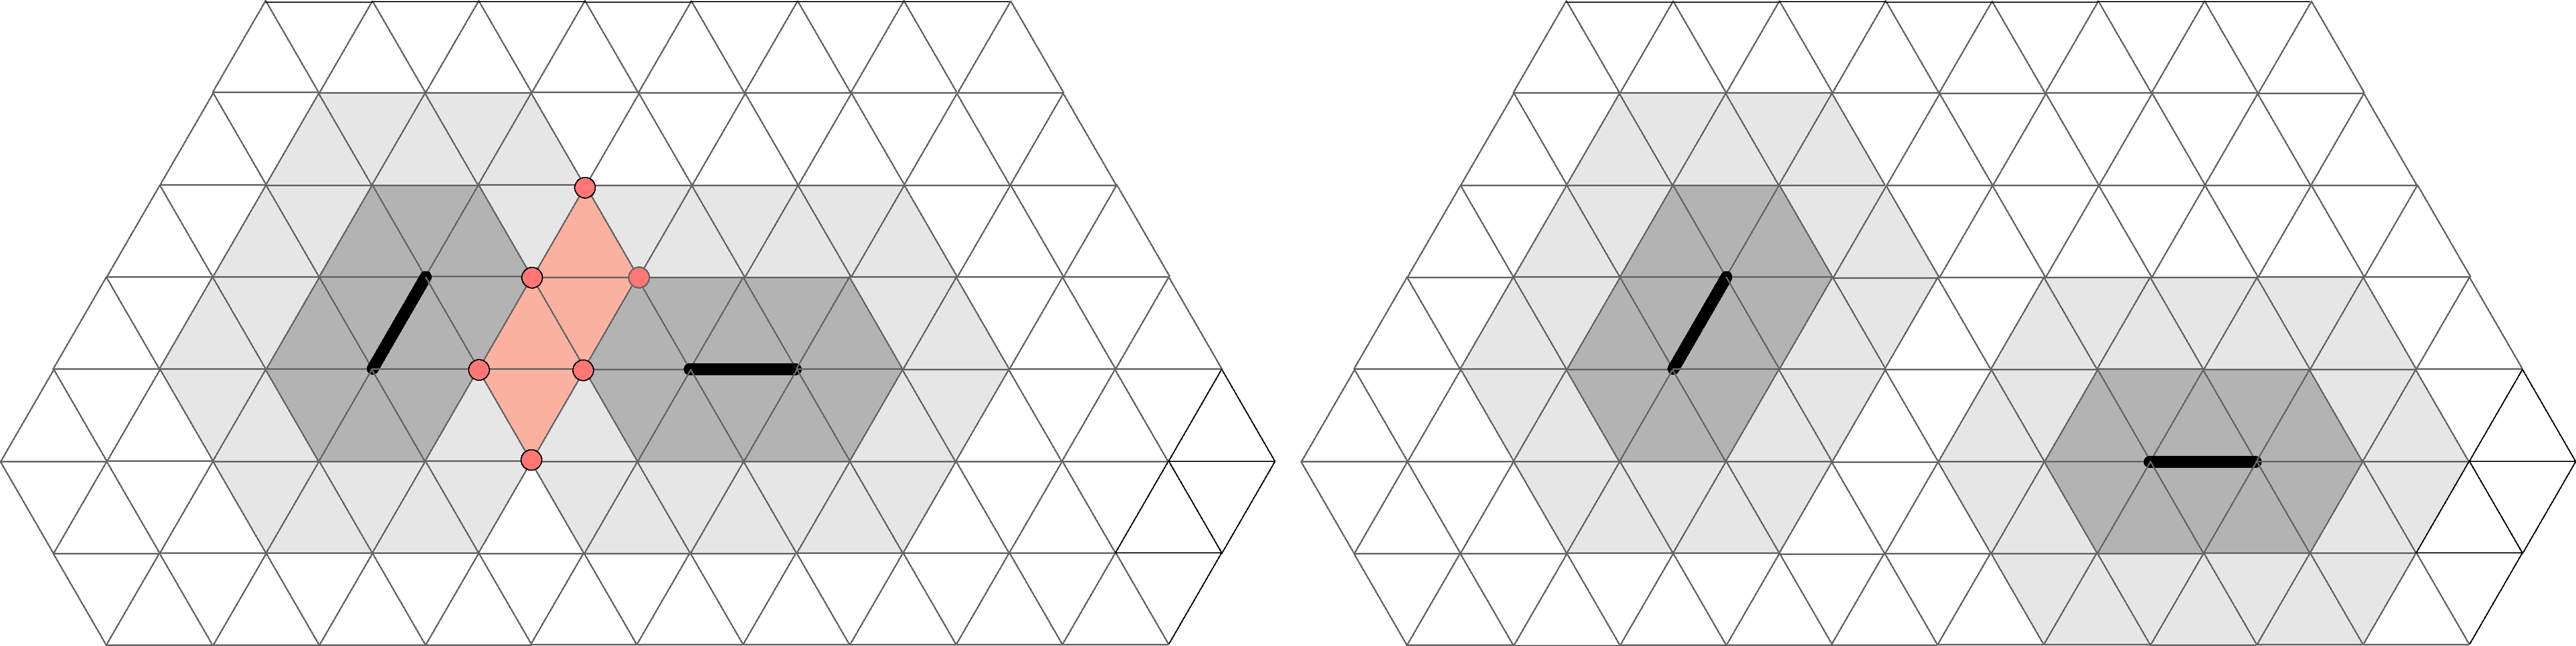
\includegraphics[width=\linewidth]{wmtk-tex/figs/lock_illustration}
    \caption{{Example of the locking region for two edges. In the example the operation requires locking a two-ring neighborhood (e.g.,  for the edge collapse operation). If the two edges are sufficiently far (right) both operations can be safely executed in parallel. When the two edges are close (left) the operations might fail acquiring the mutexes in the shared area.}}
    \label{fig:lock-example}
\end{figure}

Each mesh vertex is associated with a mutex. Whenever a thread wants to access (read/write) any attribute stored in a vertex, edge, triangle, or tetrahedron it must first acquire a lock on \emph{all} the vertices of the tetrahedron containing the element(s) storing the attribute (Figure~\ref{fig:lock-example}). For example, if a thread wants to read a value on an edge of a 3D mesh, it first needs to acquire a lock on all vertices of all the tetrahedra containing that edge. This mechanism is used also for mesh navigation, and for updating the mesh connectivity. 

At a first look, this mechanism might seem cumbersome and expensive. However, we rely on asynchronous, tentative lock acquisition operations. We \emph{try} to acquire the lock, and give up if the lock is already taken by another thread. These operations are efficient on modern hardware and dramatically improve the performance, while avoiding deadlocks. A downside is that an operation might be skipped due to impossibility of acquiring a mutex. These operations are retried for several times (by default 10 times) and run serially if the still do not succeed. Before performing any local operation, we try to acquire the lock on vertices in the 1-ring or 2-ring of the vertex involved in the operation. For example, a vertex smoothing operation requires acquiring the 1-ring vertex neighborhood of the smoothed vertex, while an edge-collapse operation on an edge $(v_1, v_2)$ requires acquiring the lock on the 2-ring vertex neighborhood of both $v_1$ and $v_2$
({Figure ~\ref{fig:lock-example}}).

Finally, since we partition the input mesh using {Morton Encoding} \cite{karras2012maximizing}, the amount of conflicts (and skipped operations) is low.



\subsection{{Example: Shortest Edge Collapse}}

We show how the library is used in a classical example, shortest edge collapse. In this case, we add a 3D position to every vertex as a vertex attribute (by default, there are no attributes attached to mesh elements). For every attribute and for every operation we plan to use in the scheduler, we need to provide a function that updates such attribute (Algorithm~\ref{algo:shortest}). In the \texttt{collapse\_before} function, we cache the two vertex coordinates associated with the collapsed edge represented by \texttt{Tuple t}. In the \texttt{collapse\_after} function, we generate a new vertex in the middle of the two endpoints of the collapsed edge. %For instance, this method can be changed to collapse to \texttt{v1p} by simply assigning \texttt{p} to \texttt{v1p}.

\begin{algorithm}
\inputminted{cpp}{wmtk-tex/code/shortest.cpp}
\caption{Overridden methods in \texttt{TriMesh} sub-class to implement shortest edge collapse.}
\label{algo:shortest}
\end{algorithm}

Equipped with the 3D position attribute, which at this point will be automatically kept up to date by the library, we can now schedule the collapse operation (Algorithm \ref{algo:shortest-sced}). For shortest edge collapse, we want to attempt to collapse all edges, prioritizing the shortest ones, until we reach a fixed number of collapses \texttt{n\_collapse}: in the code we registering the operation type (\texttt{ops}), specify how to update the queue after an operation (\texttt{renew}) by adding all the neighbouring edges, and specifying the edge length as a priority (\texttt{priority}). Note that the {outdated} elements in the queue that are affected by a local operation are automatically invalidated using a tagging mechanism on the tuples which is opaque to the user.

% TODO code too long 
\begin{longlisting}
\inputminted{cpp}{wmtk-tex/code/shortest-sched.cpp}
\caption{Scheduler setup for the schedule shortest edge collapse.}
\label{algo:shortest-sced}
\end{longlisting}